 
\section{Problem 1}
\label{part1}
\begin{verbatim}
 D3 graphing (5 points)

Use D3 to visualize your Twitter followers.  Use my twitter account
(``@phonedude_mln'') if you do not have >= 50 followers.  For example,
@hvdsomp follows me, as does @mart1nkle1n.  They also follow each
other, so they would both have links to me and links to each other.

To see if two users follow each other, see:
https://dev.twitter.com/rest/reference/get/friendships/show

Attractiveness of the graph counts!  Nodes should be labeled (avatar
images are even better), and edge types (follows, following) should
be marked.

Note: for getting GitHub to serve HTML (and other media types), see:
http://stackoverflow.com/questions/6551446/can-i-run-html-files-directly-from-github-instead-of-just-viewing-their-source

Be sure to include the URI(s) for your D3 graph in your report. 
\end{verbatim}

\subsection{Solution}

\begin{enumerate}
\item The aim of this question is to get list of followers for any account and find the friendship among the followers,i.e to find whether any followers follow each other so that they will have the links to the source account and links to each other.
\item Here I used my account ``dineshpaladhi'' because I have more than 50 followers.u.
\item So, here my first step is to get all my followers list.
\item I wrote python code for it using tweepy library and the code can be found in listing\ref{lst:q1-1}.
\item I have taken name, screen name, imageurl, and gave an id to each follower of mine. 
\item Now I have to find the friendship among all my followers, the code for this is found in listing\ref{lst:q1-2}.
\item Here I got a lot of errors like ``Rate Limit Error'', ``Not Authorized Error'',etc.
\item It took a lot of time to figure this out and I found that ``Rate Limit Error'' is because of the excess input I am giving to the program, so I broken down my input list into smaller parts and ran the program repeatedly with smaller inputs.
\item I deleted few users and their combination of friendships because they give ``Not Authorized Error'' as they have some privacy settings. This list can be found in figure\ref{Sample_list1}.
\item Later, I got all the combination of possible friendships among my users. I have 61 followers so total combinations that I got is 61*60/2 = 1830. The sample list of this can be found in figure\ref{Sample_list2}.
\item This list is then processed using the reference provided in the questions and it gave me a list of followers who follow each other. The sample list of this can be found in figure\ref{Sample_list3}.
\item The final sample json file can be seen in figure\ref{Sample_list4} and this json file is given as input to the html code which can be seen in listing\ref{lst:q1-3}.
\item The d3 graph can be seen at this link \url{http://bl.ocks.org/PaladhiDinesh/56e1843c31960ecfe919} and the sample screenshot of it can be seen in figure\ref{graph1}.
\item This is a directed graph, so we can view who follows who using the arrow mark.

\end{enumerate}

\subsection{Code Listing}

\lstinputlisting[language=Python,breaklines = true,frame=single,caption={Python code for getting twitter followers for my account }, label=lst:q1-1,captionpos=b,numbers=left,showspaces=false,showstringspaces=false,basicstyle=\footnotesize]{twit_followers.py}
\newpage

\subsection{Code Listing}

\lstinputlisting[language=Python,breaklines = true,frame=single,caption={Python code to find out friendship between my followers. }, label=lst:q1-2,captionpos=b,numbers=left,showspaces=false,showstringspaces=false,basicstyle=\footnotesize]{friendship.py}
\newpage

\subsection{Code Listing}

\lstinputlisting[language=Html,breaklines = true,frame=single,caption={HTML code with d3 to get force directed graph
 }, label=lst:q1-3,captionpos=b,numbers=left,showspaces=false,showstringspaces=false,basicstyle=\footnotesize]{followers_nodelink.html}
\newpage

\subsection{Results}

\subsubsection{Deleted Users}
\begin{figure}[ht]    
    \begin{center}
        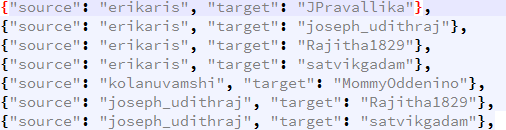
\includegraphics[scale=0.6]{sample_delete_users.png}
        \caption{Sample list of users who give not authorized error}
        \label{Sample_list1}
    \end{center}
\end{figure}

\subsubsection{Sample output1}
\begin{figure}[ht]    
    \begin{center}
        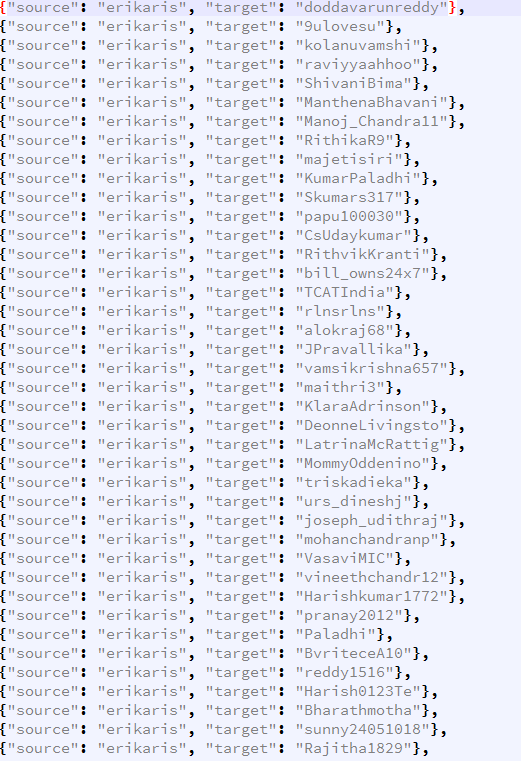
\includegraphics[scale=0.6]{sample_f1.png}
        \caption{Total combinations of possible friendship among my followers}
        \label{Sample_list2}
    \end{center}
\end{figure}
\newpage

\subsubsection{Sample output2}
\begin{figure}[ht]    
    \begin{center}
        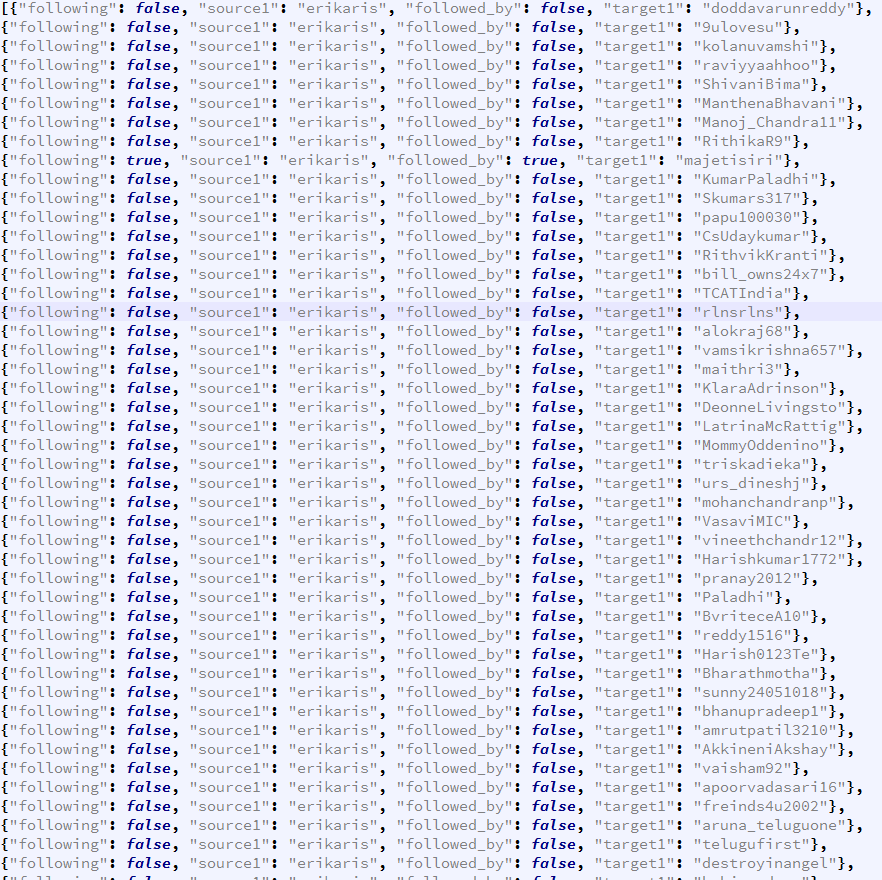
\includegraphics[scale=0.7]{sample_f2.png}
        \caption{Friendship among followers are shown here as source and target}
        \label{Sample_list3}
    \end{center}
\end{figure}
\newpage

\subsubsection{Sample final json file}
\begin{figure}[ht]    
    \begin{center}
        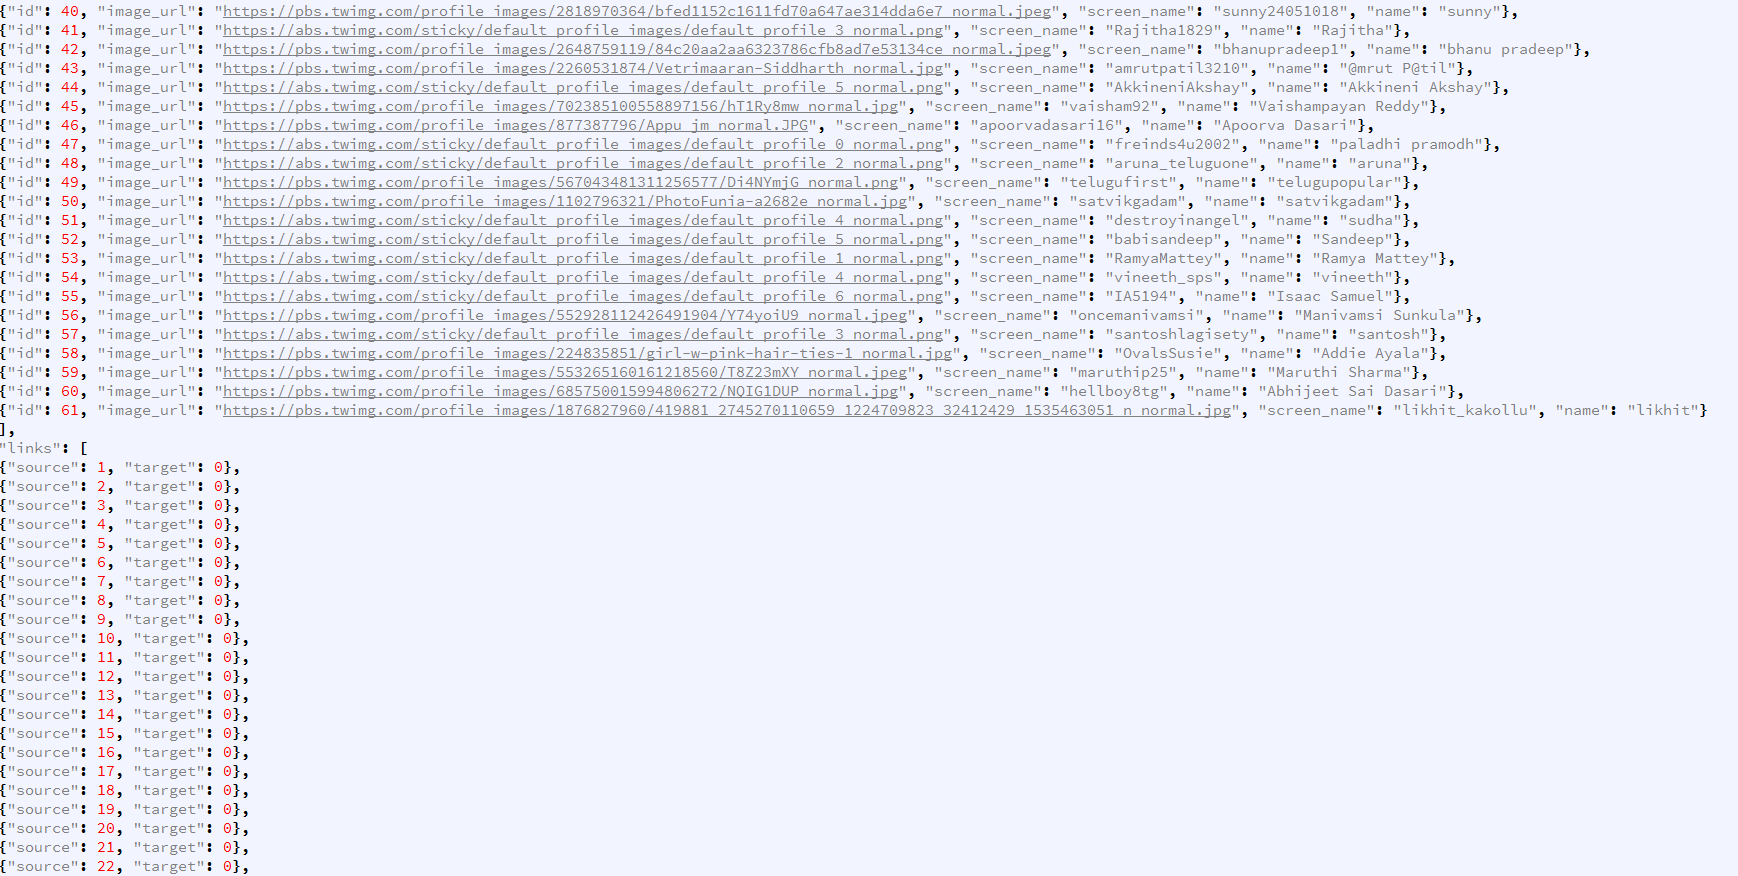
\includegraphics[scale=0.7]{sample_followers_json.png}
        \caption{Final json file with nodes as followers and links as friendship between them}
        \label{Sample_list4}
    \end{center}
\end{figure}
\newpage
\subsubsection{D3 Graph}
\begin{figure}[ht]    
    \begin{center}
        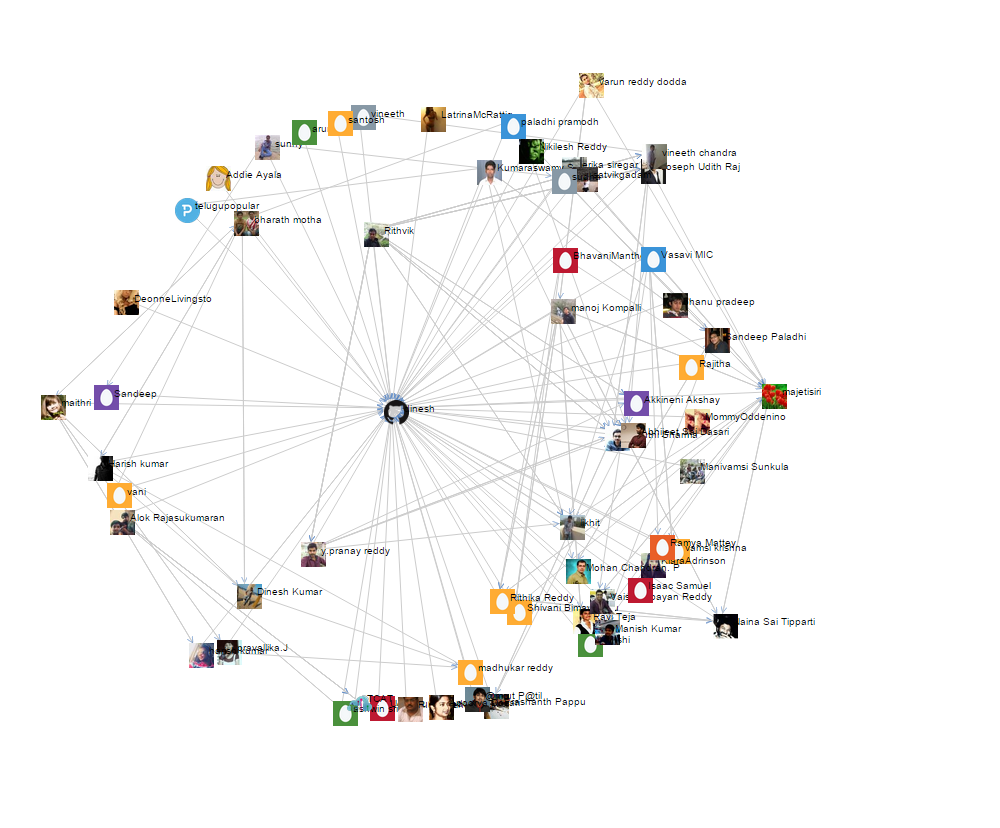
\includegraphics[scale=0.8]{q1.png}
        \caption{D3 graph showing my twitter followers and friendship among my followers}
        \label{graph1}
    \end{center}
\end{figure}
\newpage